\documentclass[12pt]{article}

% for special characters
\usepackage[utf8]{inputenc}
% for images
\usepackage{graphicx}
\graphicspath{{img/}}
% for source in images
\usepackage{floatrow}
% for urls
\usepackage{url}
% for references
\usepackage{biblatex}
\addbibresource{references.bib}

\begin{document}

\title{
\vspace{-2.0cm}

\includegraphics{zhaw}\\ 
\vspace{3cm}
Deep learning classification of rheumatoid arthritis\\
{\Large Zurich University of Applied Sciences}}
\author{\begin{tabular}{rl}
  \textbf{Author:} & Janick Rohrbach \\
  \textbf{Supervisor:} & Dr. Oliver Dürr \\ & Prof. Dr. Beate Sick \\
  \textbf{Industrial Partner:} & Seantis GmbH \\
  \textbf{External Supervisor:} & Fabian Reinhard \\ & Tobias Reinhard \\
  \textbf{Date:} & December 12, 2017
\end{tabular}}
\date{}
\maketitle

\newpage

\section*{Declaration of originality\\ \large{Project Thesis at the School of Engineering}}
By submitting this project thesis, the undersigned student confirms that this thesis is his own work and was written without the help of a third party. \\
\\
The student declares that all sources in the text (including Internet pages) and appendices have been correctly disclosed. This means that there has been no plagiarism, i.e. no sections of the project thesis have been partially or wholly taken from other texts and represented as the student’s own work or included without being correctly referenced. \\
\\
Any misconduct will be dealt with according to paragraphs 39 and 40 of the General Academic Regulations for Bachelor’s and Master’s Degree courses at the Zurich University of Applied Sciences (Rahmenprüfungsordnung ZHAW (RPO)) and subject to the provisions for disciplinary action stipulated in the University regulations.\\
\vspace{3cm} \\
City, Date: \hspace{5cm} Signature:

\newpage

\section*{Abstract}
Abstract goes here

\newpage

\section*{Acknowledgements}
I want to thank...

\newpage

\tableofcontents

\newpage

\section{Introduction}
Nennt bestehende Arbeiten/Literatur zum Thema Literaturrecherche • Stand der Technik: Bisherige Lösungen des Problems und deren Grenzen • (Nennt kurz den Industriepartner und/oder weitere Kooperationspartner und dessen/deren Interesse am Thema Fragestellung) 

Formuliert das Ziel der Arbeit • Verweist auf die offizielle Aufgabenstellung des/der Dozierenden im Anhang • (Pflichtenheft, Spezifikation) • (Spezifiziert die Anforderungen an das Resultat der Arbeit) • (Übersicht über die Arbeit: stellt die folgenden Teile der Arbeit kurz vor) • (Angaben zum Zielpublikum: nennt das für die Arbeit vorausgesetzte Wissen) • (Terminologie: Definiert die in der Arbeit verwendeten Begriffe) 

\section{Chapter Two Title}
\subsection{Rheumatoid arthritis}
\label{subsec:rheuma}

Rheumatoid arthritis is caused by a malfunctioning immune system. The immune attacks healthy tissue instead of bacteria and viruses. This causes inflammation in the joints. Irreversible damage to the joint can occur, if the inflammation lasts for a long time. \cite{rheuma}

\subsection{Convolutional neural networks}
\label{subsec:cnn}
Convolutional neural networks take an image as an input. The image then gets passed through several convolutional layers. These layers work as filters and detect different features in the image. The weights of these layers are combined to class scores. Andrey Karpathy provides a good overview over convolutional neural networks in his course notes for the Stanford class CS231n. \cite{cnn}

\subsection{Rau classification}
\label{subsec:rau}

\begin{figure}
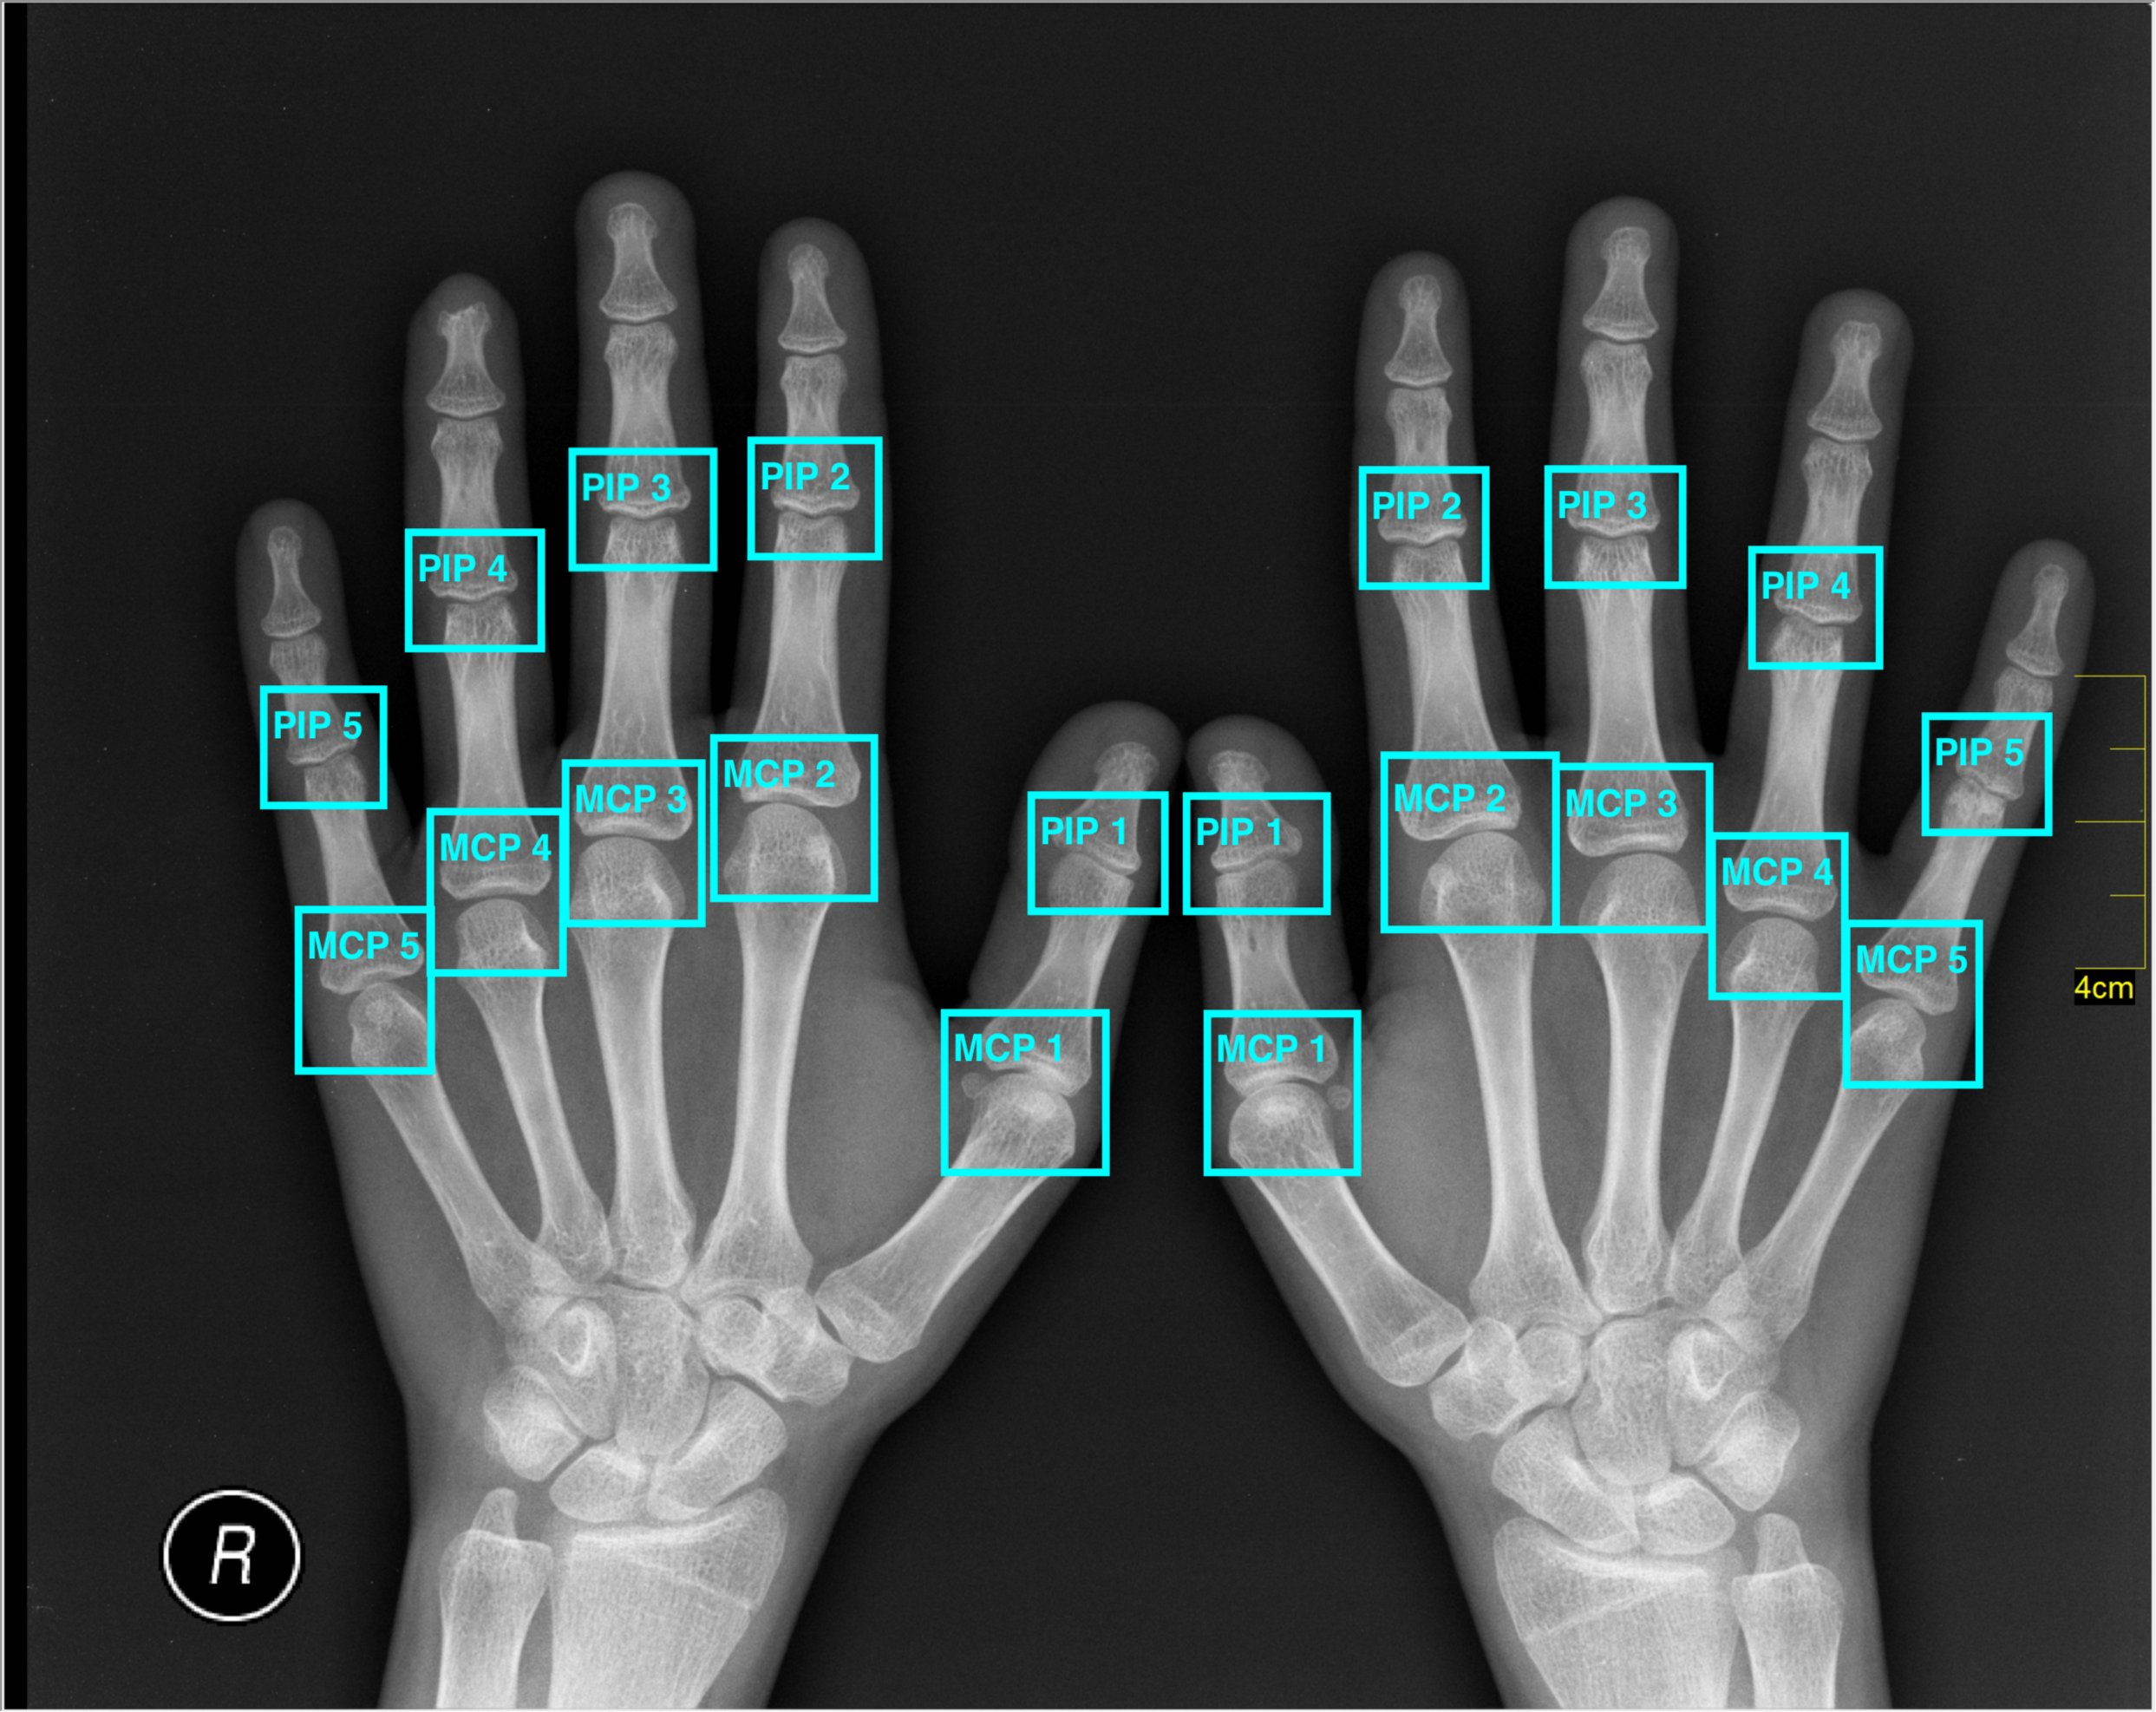
\includegraphics[width=10cm]{labels}	
\caption{Proximal interphalangeal joints (PIP) and carpometacarpal joints (MCP).}
\floatfoot{Image by Nevit Dilmen (CC BY-SA) \url{https://commons.wikimedia.org/wiki/File:Medical\_X\-Ray\_imaging\_OPC06\_nevit.jpg}}
\label{fig:labels}
\end{figure}



\section{Chapter Three Title}


\section{Chapter Four Title}


\section{Conclusion}







\newpage
\printbibliography

\newpage
\listoffigures


\end{document}
